\subsection{Непрерывная дифференцируемость}

\begin{theorem}
    Пусть $f: E\rightarrow \R$, $E\subset \R^n$, $a\in \Int E$. Если все частные производные функции $f$ непрерывны в точке $a$, то $f$  дифференцируема в точке $a$.
\end{theorem}

\begin{proof}
    Пусть $R(h):=f(a + h) - f(a) - \sum\limits_{k=1}^n\pdv{f}{x_k}(a) h_k$. Надо доказать, что $R(h)=o(\|h\|)$ при $h\rightarrow 0$ .

    $b_k =\begin{pmatrix}
        a_1 + h_1 \\ \vdots \\ a_k + h_k \\ a_{k+1} \\ \vdots \\ a_n
    \end{pmatrix}\quad f(a+h)-f(a)=\sum\limits_{k=1}^n(f(b_k) - f(b_{k-1}))\overset{(*)}{=}$

    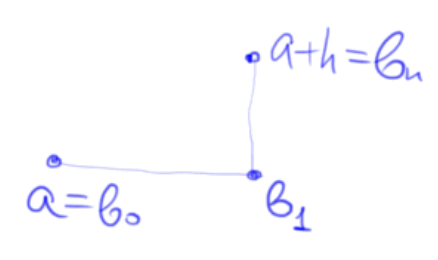
\includegraphics[width=0.25\linewidth]{images/24-05-1.png}

    $a=b_0$, $a+h=b_n\quad F_{k-1}(t) := f(b_{k-1} + th_ke_k)$

    $f(b_k) - f(b_{k-1})=F_{k-1}(1)- F_{k-1}(0)=$ (по th Лагранжа) $= \underset{\Theta_k\in (0, 1)}{F'_{k-1}(\Theta_k)}=$ (производная композиции) $=\begin{pmatrix}
    \frac{\partial f}{\partial x_1}(b_{k-1} + \Theta_kh_ke_k) & ... & \frac{\partial f}{\partial x_n}(b_{k-1} + \Theta_kh_ke_k)
    \end{pmatrix}\cdot \begin{pmatrix}
        0 \\ \vdots \\ 0 \\ h_k \\ \vdots \\ 0
    \end{pmatrix}=h_k\cdot \frac{\partial f}{\partial x_k}(b_{k-1} + \Theta_kh_ke_k)$

    $\overset{(*)}{=}\sum\limits_{k=1}^n h_k  \frac{\partial f}{\partial x_k} (a) + \underset{\leq \|h\|\cdot \|... \|}{\underbrace{\sum\limits_{k=1}^n h_k (\underbrace{\frac{\partial f}{\partial x_k}(b_{k-1} + \Theta_kh_ke_k)-\frac{\partial f}{\partial x_k}(a)}_{\underset{h\rightarrow 0}{\rightarrow} 0})}_{=o(\|h\|)}}$ ($b_k$-шки стремятся к $a$ и по непрерывности в точке $a$ коэффициент перед каждым $h_k$ стремится к 0)

    $F_0(1)-F_0(0)= f(a + h_1e_1) - f(a) = h\frac{\partial f}{\partial x_1}(a) + o(h_1)$ – определение дифференцируемости $F_0$ в точке $a$.
\end{proof}

\begin{remark}~
    \begin{enumerate}
        \item Теорема верна и без непрерывности $\pdv{f}{x_1}$ в точке $a$. Достаточно только ее существования.
        \item Обратное утверждение неверно. Дифференцируемость функции в точке $a$ не гарантирует даже непрерывности в окрестности $a$, а также сущестовования хоть каких-то частных производных.

        \begin{example}
            $f(x, y)=\left\{\begin{array}{ll}
                x^2 + y^2, & \text{ если ровно одно из чисел $x$ и $y$ рационально;} \\
                0, & \text{ иначе.}
            \end{array}\right.$

            $f$  дифференцируема в точке $(0, 0)$

            $f(h, k)=o(\sqrt{h^2+k^2})$

            $f(0, 0)=0$, линейное отображение $\equiv 0$.
        \end{example}
    \end{enumerate}
\end{remark}

\begin{definition}
    $f$ \textit{непрерывно дифференцируема в точке $a$}, если $f$ дифференцируема в окрестности точки $a$ и $\|d_xf-d_af\|\underset{x\rightarrow a}{\rightarrow} 0$.
\end{definition}

\begin{theorem}
    Пусть $f: E\rightarrow \R^m$, $E\subset \R^n$, $a\in \Int E$, $f$ дифференцируема в окрестности точки $a$. Тогда $f$ непрерывно дифференцируема в точке $a\Leftrightarrow\pdv{f_i}{x_j}$ непрерывна в точке $a$ $\forall i, j$. 
\end{theorem}
\begin{proof}~
    \begin{enumerate}
        \item[$\Leftarrow$.]  Проверим непрерывность:
        
        $\|d_xf - d_af\|^2\leq \sum\limits_{i=1}^n\sum\limits_{k=1}^m\underbrace{(\frac{\partial f_k}{\partial x_i}(x)-\frac{\partial f_k}{\partial x_i}(a))^2}_{\underset{x\rightarrow a}{\rightarrow} 0}\underset{x\rightarrow a}{\rightarrow} 0$

        $f'(x)-f'(a)=\begin{pmatrix}
            \frac{\partial f_1}{\partial x_1}(x)-\frac{\partial f_1}{\partial x_1}(a) & ... & \frac{\partial  f_1}{\partial x_n}(x)-\frac{\partial f_1}{\partial x_n}(a) \\
            \vdots & \ddots & \vdots \\
            \frac{\partial f_m}{\partial x_1}(x)-\frac{\partial f_m}{\partial x_1}(a) & ... & \frac{\partial f_m}{\partial x_n}(x)-\frac{\partial f_m}{\partial x_n}(a) 
        \end{pmatrix}$
        \item[$\Rightarrow$.] $|\frac{\partial f_k}{\partial x_i}(x)-\frac{\partial f_k}{\partial x_i}(a)|\leq \|\begin{pmatrix}
            \frac{\partial f_1}{\partial x_i}(x)-\frac{\partial f_1}{\partial x_i}(a) \\
            \vdots \\
            \frac{\partial f_m}{\partial x_i}(x)-\frac{\partial f_m}{\partial x_i}(a)
        \end{pmatrix}\|=\|(d_xf-d_af)(e_i)\|\leq \underbrace{\|d_x f-d_af\|}_{\rightarrow 0}\underbrace{\|e_i\|}_{=1}$, $e_i=\begin{pmatrix}
            0 \\ \vdots \\ 1 \\ \vdots \\ 0
        \end{pmatrix}$
    \end{enumerate}
\end{proof}

\begin{theorem}
    Непрерывная дифференцируемость сохраняется при линейной комбинации, скалярном произведении, композиции.
\end{theorem}


\subsection{Частные производные высших порядков}

\begin{definition}
    Пусть $f: E\rightarrow \R$, $E\subset \R^n$, $a\in \Int E$ и в окрестности точки $a$ существует $\pdv{f}{x_i}: \text{ окр-ть точки $a$ }\rightarrow \R$. Если у $\pdv{f}{x_i}$ существует частная производная по $x_j$, то результат $\frac{\partial^2 f}{\partial x_j\partial x_i}$ – это \textit{вторая частная производная по $x_j$} (нужно уточнение, по какой переменной).

    Обозначения: $\frac{\partial^2 f}{\partial x_j\partial x_i}$, $f''_{x_ix_j}$, $\frac{\partial}{\partial x_j}(\frac{\partial f}\partial x_i)$, $(f'_{x_i})'_{x_j}$.

    $\frac{\partial^r f}{x_{i_r}...\partial x_{i_1}}$ – \textit{частная производная порядка $r$}.
\end{definition}

\begin{remark}
    Всего $n^r$ производных $r$-ого порядка.
\end{remark}

\begin{example}
    $f(x, y) = x^y$, где $x, y>0$.

    $f'_x(x, y)=yx^{y-1}$, $f'_y(x, y)=x^y\ln x$

    $f''_{xx}(x, y)=(yx^{y-1})'_x=y(y-1)x^{y-2}$
    
    $f''_{yy}(x, y)=(x^y\ln x)'_y=\ln^2x\cdot x^y$

    $f''_{xy}(x, y)=(yx^{y-1})'_y=yx^{y-1}\cdot \ln x+x^y\cdot\frac{1}{x}$

    $f''_{yx}(x, y)=(x^y\ln x)'_x=yx^{y-1}\cdot \ln x+x^y\cdot \frac{1}{x}$

    Заметим, что $f''_{xy}(x, y)=f''_{yx}(x, y)$.
\end{example}

\begin{example}
    $f(x, y)=\left\{\begin{array}{ll}
        xy\cdot\frac{x^2-y^2}{x^2+y^2}, & \text{ при $x^2+y^2\neq 0$} \\

        0, & \text{ при $x=y= 0$}
    \end{array}\right.$

    $f'_x(x, y)=y\cdot \frac{x^2-y^2}{x^2+y^2}+xy\cdot \frac{2x(x^2+y^2)-2x(x^2-y^2)}{(x^2+y^2)^2}$

    $f'_x(0, 0)=\lim\limits_{h\rightarrow 0}\frac{f(h, 0)-f(0, 0)}{h}=0$

    $f''_{xy}(0, 0)=\lim\limits_{h\rightarrow 0}\frac{f'_x(0, h)-f'_x(0, 0)}{h}=\lim\limits_{h\rightarrow 0}\frac{-h}{h}=-1$

    $f''_{yx}(0, 0)=1$ (меняется знак исходного выражения) $\Rightarrow f''_{xy}(0, 0)\neq f''_{yx}(0, 0)$
\end{example}

\begin{theorem}
    Пусть $f: E\rightarrow \R$, $E\subset \R^2$, $(x_0, y_0)\in \Int E$ и в окрестности точки $(x_0, y_0)$ существуют $f'_x$, $f'_y$ и $f''_{xy}$. Тогда если $f''_{xy}$ непрерывна в точке $(x_0, y_0)$, то $f''_{yx}$ существует в точке $(x_0, y_0)$ и $f''_{xy}(x_0, y_0)=f''_{yx}(x_0, y_0)$.
\end{theorem}
\begin{proof}
    Пусть $\varphi(s):= f(s, y_0 + k)-f(s, y_0)$ – дифференцируема, так как у $f$  существует производная по первой координате.
    
    $\varphi(x_0+h)-\varphi(x_0)=h\varphi'(x_0+\Theta h)\underset{\text{где }\Theta\in (0, 1)}{=}h(f'_x(x_0+\Theta h, y_0+k)-f'_x(x_0+\Theta h, y_0))=$ (теперь функция дифференцируема по второй координате) $\underset{\text{где $\Tilde{\Theta}\in (0, 1)$}}{=}hkf''_{xy}(x_0+\Theta h, y_o+\Tilde{\Theta}k)=hk(f''_{xy}(x_0, y_0)+\alpha(h, k))$, где $\alpha(h, k)\underset{(h, k)\rightarrow 0}{\rightarrow}0$
    
    $\forall \varepsilon>0$ при $(h, k)$ близких к $(0, 0)$: $|\frac{\varphi(x_0+h)-\varphi(x_0)}{hk}-f''_{xy}(x_0, y_0)|<\varepsilon$

    $\frac{\varphi(x_0)}{k}=\frac{f(x_0, y_0 + k) - f(x_0, y_0)}{k}\rightarrow f'_y(x_0, y_0)$

    $|\frac{1}{h}(\frac{\varphi(x_0+h)}{k}-\frac{\varphi(x_0)}{k})-f''_{xy}(x_0, y_0)|\rightarrow |\frac{1}{h}(f'_y(x_0 + h, y_0) - f'_y(x_0, y_0))-f''_{xy}(x_0, y_0)|\leq \varepsilon$ (перешли к пределу)

    $\Rightarrow$ при $h$ близких к нулю $|\frac{f'_y(x_0 + h, y_0) - f'_y(x_0, y_0)}{h} -f''_{xy}(x_0, y_0)|< \varepsilon\Rightarrow \underset{=f''_{yx}(x_0, y_0)\text{ по опр.}}{\lim\limits_{h\rightarrow 0}\frac{f'_y(x_0 + h, y_0) - f'_y(x_0, y_0)}{h}}=f''_{xy}(x_0, y_0)$

\end{proof}

\begin{exercise}
    Если $f'_x$ и $f'_y$ определены в окрестности точки $(x_0, y_0)$ и дифференцируемы в этой точке, то $f''_{xy}(x_0, y_0)=f''_{yx}(x_0, y_0)$.
\end{exercise}

\begin{definition}
    Пусть $f:D\rightarrow \R$, $D\subset \R^n$, $D$ открыто. Тогда $f$ – это \textit{$r$ раз непрерывно дифференцируемая в $D$ функция} (\textit{$r$-гладкая функция в $D$}),  если все частные производные до $r$-ого порядка включительно существуют и непрерывны.

    \textit{Обозначение:} $f\in C^r(D)$.
\end{definition}

\begin{theorem}
    Пусть $f:D\rightarrow \R$, $D\subset \R^n$, $D$ открыто, $f\in C^r(D)$ и $(i_1, i_2, ..., i_r)$ – перестановка $(j_1, j_2, ..., j_r)$. Тогда $\frac{\partial^r f}{\partial x_{i_1} \partial x_{i_2} ... \partial x_{i_r}}=\frac{\partial^r f}{\partial x_{j_1} \partial x_{j_2} ... \partial x_{j_r}}$.
\end{theorem}

\begin{proof}
    Любая перестановка получается с помощью какого-то количества транспозиций, то есть достаточно доказать для элементарных транспозиций: $(j_1, ..., j_{k-1}, j_{k+1}, j_k, j_{k+2}, ... j_r)$.

    Пусть $g:=\frac{\partial^{r-k-1} f}{\partial x_{j_{k+2}}... \partial x_{j_r}}$. 
    
    По теореме: $\frac{\partial^2 g}{\partial x_{j_k}\partial x_{j_{k+1}}}=\frac{\partial^2 g}{\partial x_{j_{k+1}}\partial x_{j_{k}}}\Rightarrow \frac{\partial^{k+1} g}{\partial x_{j_{1}}...\partial x_{j_{k+1}}}=\frac{\partial^{k+1} g}{\partial x_{j_{1}}...\partial x_{j_{k-1}}\partial x_{j_{k+1}}\partial x_{j_{k}}}$
    
    $\Rightarrow \frac{\partial^r f}{\partial x_{j_1} \partial x_{j_2} ... \partial x_{j_r}}=\frac{\partial^r f}{\partial x_{j_1} ...\partial x_{j_{k-1}}\partial x_{j_{k+1}}\partial x_{j_k} ... \partial x_{j_r}}$.
\end{proof}

\subsection*{Приложения частных производных}
\begin{definition}
    \textit{Мультииндекс} $k=(k_1, k_2, ..., k_n)$, где $k_1, k_2$, ..., $k_n$ – неотрицательные числа.

    \textit{Высота мультииндекса} $|k|:=k_1+...+k_n$.

    $k!:=k_1!...k_n!$

    Если $h\in \R^n$, то $h^k:=h_1^{k_1}...h_n^{k_n}$.

    $f^{(k)}:=\frac{\partial^{|k|}f}{(\partial x_1)^{k_1}...(\partial x_n)^{k_n}}$
\end{definition}

\begin{definition}
    \textit{Полиномиальный (мультиномиальный) коэффициент} – $\binom{|k|}{k_1, ..., k_n}=\frac{|k|!}{k!}$. 
    
    Количество способов покрасить $|k|$ шариков в $n$ цветов так, что будет $k_i$ шариков $i$-ого цвета.

    $\binom{|k|}{k_1}\cdot \binom{|k| - k_1}{k_2}\cdot ... \cdot \binom{|k|-k_1-...-k_{n-2}}{k_{n-1}}=\frac{|k|!}{k_1!(|k|-k_1)!}\cdot \frac{(|k|-k_1)!}{k_2!(|k|-k_1-k_2)!}\cdot \frac{(|k|-k_1-k_2)!}{k_3!(|k|-k_1-k_2-k_3)!}\cdot ...=\frac{|k|!}{k_1!k_2!...k_n!}=\frac{|k|!}{k!}$
\end{definition}

\begin{lemma}
    Пусть $f\in C^r(D)$, $D\subset \R^n$ открыто, $[x_0, x_0 + h]\subset D$, $F(t):=f(x_0 + th)$, $F:[0, 1]\rightarrow \R$. Тогда $F\in C^r[0, 1]$ и $F^{(l)}(t)=\sum\limits_{|k|=l}\binom{l}{k_1, ..., k_n}f^{(k)}(x+th)\cdot h^k$.

    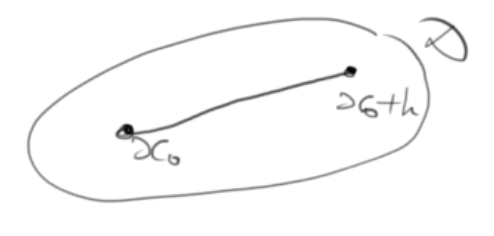
\includegraphics[width=0.2\linewidth]{images/24-05-2.png}
\end{lemma}

\begin{proof}
    Пусть $G(t)=g(x_0+th)$, $g: \R^n \rightarrow \R$ 
    
    $G'(t)=(g'_{x_1}(x_0+th)\ ...\ g'_{x_n}(x_0+th))\begin{pmatrix}
        h_1 \\ h_2 \\ \vdots \\ h_n 
    \end{pmatrix}=\sum\limits_{i=1}^n g'_{x_i}(x_0+th)h_i$

    Применим это знание и будем брать производную $F^{(l)}$ как производную $(F^{(l-1)})'$.

    $F^{(l)}(t)=\sum\limits_{i_1=1}^n...\sum\limits_{i_l=1}^n\frac{\partial ^l f}{\partial x_{i_1} ... \partial x_{i_l}}(x_0+th)h_{i_1}h_{i_2}...h_{i_l}=\sum\limits_{|k|=l}\binom{|k|}{k_1, ..., k_n}f^{(k)}(x_0+th)h^k$.

    $k=(k_1, ..., k_n)$, где $k_j=\#\{ i_p\mid i_p = j\}$
\end{proof}

\begin{theorem}
    \textbf{Многомерная формула Тейлора с остатком в форме Лагранжа}

    Пусть $D\subset \R^n$ открытое, $f\in C^{r+1}(D)$, $[a, x]\subset D$. Тогда существует $\Theta\in (0, 1)$:
    
    $f(x)=\sum\limits_{|k|\leq r}\frac{f^{(k)}(a)}{k!}(x-a)^k+\sum\limits_{|k|=r+1}\frac{f^{(k)}(a+\Theta(x-a))}{k!}(x-a)^k$.
\end{theorem}

\begin{proof}
    $h=x-a$, $F(t)=f(a+th)\Rightarrow F\in C^{r+1}[0, 1]\Rightarrow $
    
    $\Rightarrow F(1)=\sum\limits_{l=0}^r\frac{F^{(l)}(0)}{l!}\cdot 1^l+\underset{\text{где }\Theta\in (0, 1)}{\frac{F^{(r+1)}(\Theta)}{(r+1)!}\cdot 1^{r+1}}=\sum\limits_{l=0}^r\frac{1}{l!}\sum\limits_{|k|=l}\binom{l}{k_1, ..., k_n} f^{(k)}(a)h^k+\frac{1}{(r+1)!}\sum\limits_{|k|=r+1}\binom{r+1}{k_1, ..., k_n}f^{(k)}(a+\Theta h)h^k\overset{(*)}{=}\sum\limits_{l=0}^r\sum\limits_{|k|=l}\frac{f^{(k)}(a)}{k!}h^k+\sum\limits_{|k|=r+1}\frac{f^{(k)}(a+\Theta h)}{k!}h^k$.

    $(*):$ $\frac{1}{l!}\binom{l}{k_1, ..., k_n}=\frac{1}{k!}$
\end{proof}

\begin{remark}~
    \begin{enumerate}
        \item $\sum\limits_{|k|\leq r}\frac{f^{(k)}(a)}{k!}(x-a)^k$ – \textit{многочлен Тейлора степени $r$}.
        \item Если $r=0$, то получаем аналог теоремы Лагранжа:

        $f(x)=f(a)+\sum\limits_{i=1}^n f'_{x_i}(a+\Theta(x-a))(x_i-a_i)=f(a)+\langle \triangledown f(a+\Theta(x-a), x-a) \rangle$
    \end{enumerate}
\end{remark}

\begin{theorem}
    \textbf{Формула Тейлора с остатком в форме Пеано.}

    Пусть $D\subset \R^n$ открытое, $f\in C^{r}(D)$, $a\in D$. Тогда при $x\rightarrow a$:
    
    $f(x)=\sum\limits_{|k|\leq r}\frac{f^{(k)}(a)}{k!}(x-a)^k+o(\|x-a\|^r)$
\end{theorem}

\begin{proof}
    Пишем формулу с остатком в форме Лагранжа для $r-1$:

    $f(x)=\sum\limits_{|k|\leq r-1}\frac{f^{(k)}(a)}{k!}(x-a)^k+\sum\limits_{|k|=r}\frac{f^{(k)}(a+\Theta (x-a))}{k!}(x-a)^k=\sum\limits_{|k|\leq r}\frac{f^{(k)}(a)}{k!}(x-a)^k+$
    
    $+\underbrace{\sum\limits_{|k|=r}(\frac{f^{(k)}(a+\Theta (x-a))-\frac{f^{(k)}(a)}{k!}}{k!})(x-a)^k}_{o(\|x-a\|^r)}$

    Пусть $h=x-a$: $f^{(k)}(a+\Theta h)-f^{(k)}(a)\underset{h\rightarrow 0}{\rightarrow}0 $. Надо понять, что $|h^k|\leq \|h\|^r$: 
    
    $|h_1^{k_1}...h_n^{k_n}|\leq \|h\|^{k_1}\cdot ... \cdot \|h\|^{k_n}=\|h\|^r$.
\end{proof}

\begin{statement}
    \textbf{Полиномиальная формула}
    
    $(x_1+x_2+...+x_n)^r=\sum\limits_{|k|=r}\binom{r}{k_1, ..., k_n}x_1^{k_1}...x_n^{k_n}=\sum\limits_{|k|=r}\frac{r!}{k!}x^k$.
\end{statement}

\begin{proof}
    $f(x_1, ..., x_n)=(x_1+...x_n)^r=g^r(x)$, где $g(x)=x_1+...x_n$.

    $\pdv{f}{x_i}=rg^{r-1}(x)\frac{\partial g}{\partial x_1}(x)=rg^{r-1}(x)$

    $f(x)=\sum\limits_{|k|\leq r}\frac{f^{(k)}(0)}{k!}x^k=\sum\limits_{|k|=r}\frac{f^{(k)}(0)}{k!}x^k=\sum\limits_{|k|=r}\frac{r!}{k!}x^k$
\end{proof}